\subsection{Graph 3}\label{Graph3}

This graph is a representation of all the data. The idea is to have one big graph that we could fitler information from.

Data insertion is showcased with the function bellow.
\begin{listing}[H]
\caption{Mega graph -part 1}
\begin{minted}{Python}
def create_mega_graph(mega_dataframe):
    uri, user, password = get_creds(2)
    driver = GraphDatabase.driver(uri, auth=(user, password))

    create_user_query = "MERGE (:User {id: $userId})"
    create_country_query = "MERGE (:Country {name: $country})"
    create_team_query = "MERGE (:Team {id: $teamId, name: $name})"
    create_platform_query = "MERGE (:PlatformType {name: $platformType})"
    create_ad_query = "MERGE (:Ad {id: $adId})"
    create_category_query = "MERGE (:AdCategory {name: $adCategory})"
    create_country_user_rel_query = 
        "MATCH (u:User), (c:Country) WHERE 
            u.id = $userId AND 
            c.name = $country CREATE (u)-[:BELONGS_TO_COUNTRY]->(c)"
    create_team_user_rel_query = 
        "MATCH (u:User), (t:Team) WHERE 
            u.id = $userId AND 
            t.id = $teamId CREATE (u)-[:MEMBER_OF_TEAM {strength: $strength}]->(t)"
    create_platform_user_rel_query = 
        "MATCH (u:User), (p:PlatformType) WHERE 
            u.id = $userId AND 
            p.name = $platformType CREATE (u)-[:USES_PLATFORM]->(p)"
    create_ad_user_rel_query = 
        "MATCH (u:User), (a:Ad) WHERE 
            u.id = $userId AND 
            a.id = $adId CREATE (u)-[:VIEWED_AD]->(a)"
    create_category_ad_rel_query = 
        "MATCH (a:Ad), (c:AdCategory) WHERE 
            a.id = $adId AND 
            c.name = $adCategory CREATE (a)-[:BELONGS_TO_CATEGORY]->(c)"
\end{minted}
\end{listing}

\begin{listing}[H]
\caption{Mega graph -part 2}
\begin{minted}{Python}
    queries = [
        (create_user_query, 
            mega_dataframe.select("userId")
            .distinct()),
        (create_country_query, 
            mega_dataframe.select("country")
            .distinct()),
        (create_team_query, 
            mega_dataframe
            .select("teamId", "name")
            .distinct()),
        (create_platform_query, 
            mega_dataframe
            .select("platformType")
            .distinct()),
        (create_ad_query, 
            mega_dataframe
            .select("adId")
            .distinct()),
        (create_category_query, 
            mega_dataframe
            .select("adCategory")
            .distinct()),
        (create_country_user_rel_query, 
            mega_dataframe
            .select("userId", "country")),
        (create_team_user_rel_query, 
            mega_dataframe
            .select("userId", "teamId", "strength", "name")),
        (create_platform_user_rel_query, 
            mega_dataframe
            .select("userId", "platformType")),
        (create_ad_user_rel_query, 
            mega_dataframe
            .select("userId", "adId")),
        (create_category_ad_rel_query, 
            mega_dataframe
            .select("adId", "adCategory"))
    ]

    with driver.session() as session:
        for query, data in queries:
            for row in data.collect():
                session.run(query, **row.asDict())
\end{minted}
\end{listing}

\begin{landscape}
    \begin{figure}[H]
        \includegraphics[scale=0.109]{img/Neo4j/graph2.png}
        \centering
        \caption{Graph 3}
        \label{fig:graph2}
    \end{figure}
\end{landscape}

We can filter out couturiers with most of the users.
\begin{listing}[H]
\caption{Cypher filter 3}
\begin{minted}{Cypher}
MATCH (n)-[r:BELONGS_TO_COUNTRY]->()
WITH n, COUNT(r) AS belongsToCountryCount
ORDER BY belongsToCountryCount DESC
LIMIT 10
MATCH (n)-[rel]->(m)
RETURN n, rel, m
\end{minted}
\end{listing}

\begin{landscape}
  \begin{figure}[H]
    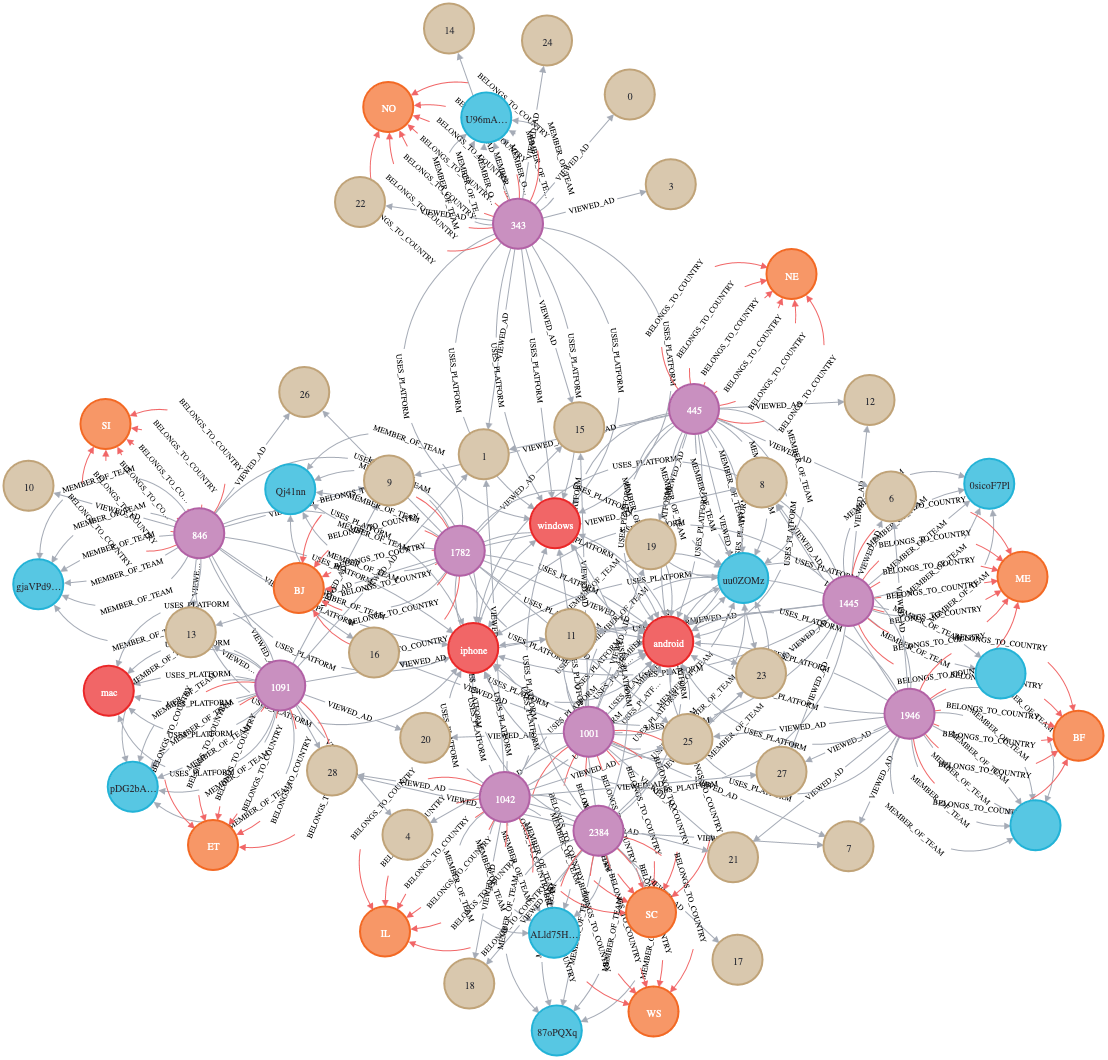
\includegraphics[scale=0.37]{img/Neo4j/graph2-filter.png}
    \centering
    \caption{Graph 3 filtered}
    \label{fig:graph0}
  \end{figure}
\end{landscape}